\begin{figure}[htbp]
  \centering
  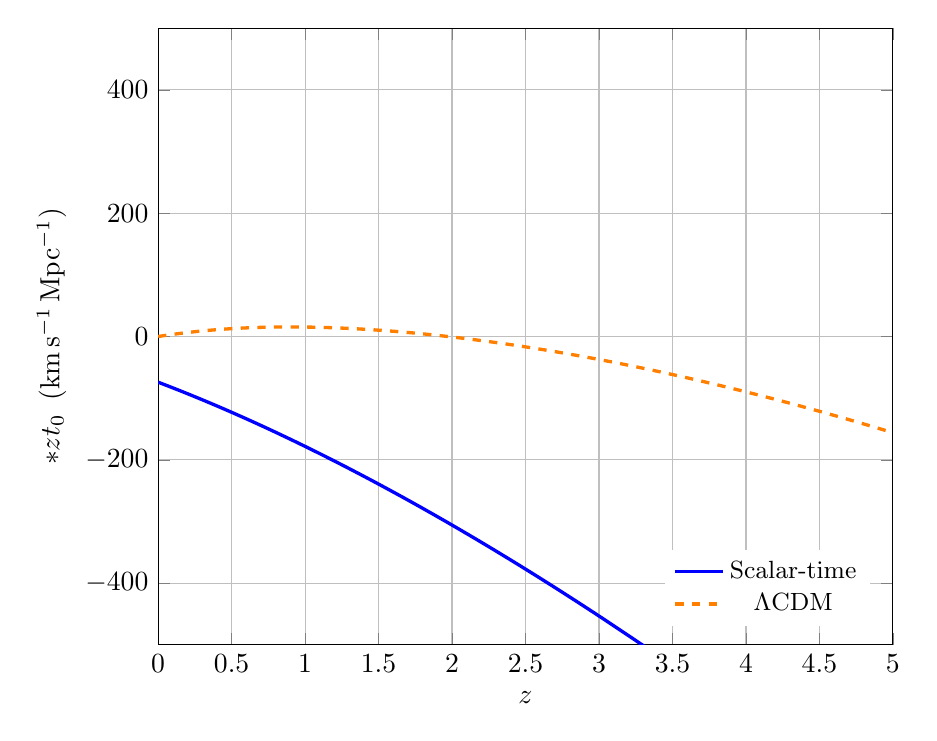
\begin{tikzpicture}
  \begin{axis}[
      width=0.9\textwidth,
      xlabel={$z$},
      ylabel={$\dv*{z}{t_0}$ \,(km\,s$^{-1}$\,Mpc$^{-1}$)},
      xmin=0, xmax=5,
      ymin=-500, ymax=500,
      grid=both,
      legend style={draw=none, font=\small},
      legend pos=south east]
    \addplot[blue,very thick,domain=0:5,samples=250]
      {-70*sqrt(0.50*(1+x)^3 + 0.62*(1+x)^2 + 4.2e-5*(1+x)^4)};
    \addlegendentry{Scalar-time}
    % --- ΛCDM  --------------------------------------------------
    \addplot[orange,dashed,very thick,domain=0:5,samples=250]
      {(1+x)*70 - 70*sqrt(0.31*(1+x)^3 + 0.69 + 4.2e-5*(1+x)^4)};
    \addlegendentry{$\Lambda$CDM}
  \end{axis}
  \end{tikzpicture}
  %-------------------------------------------------------------
  \caption{Predicted red-shift drift $\dv*{z}{t_{0}}$ for the scalar-time model (solid blue) and $\Lambda$CDM (dashed orange).  At $z\!\simeq\!2$ the two curves differ by the equivalent of $\sim6$\,cm\,s$^{-1}$\,yr$^{-1}$, a signal reachable by ELT-HIRES in the 2030s.}
  \label{fig:RedshiftDrift}
\end{figure}
